\begin{figure*}[t]
\centering
\resizebox{\textwidth}{!}{%
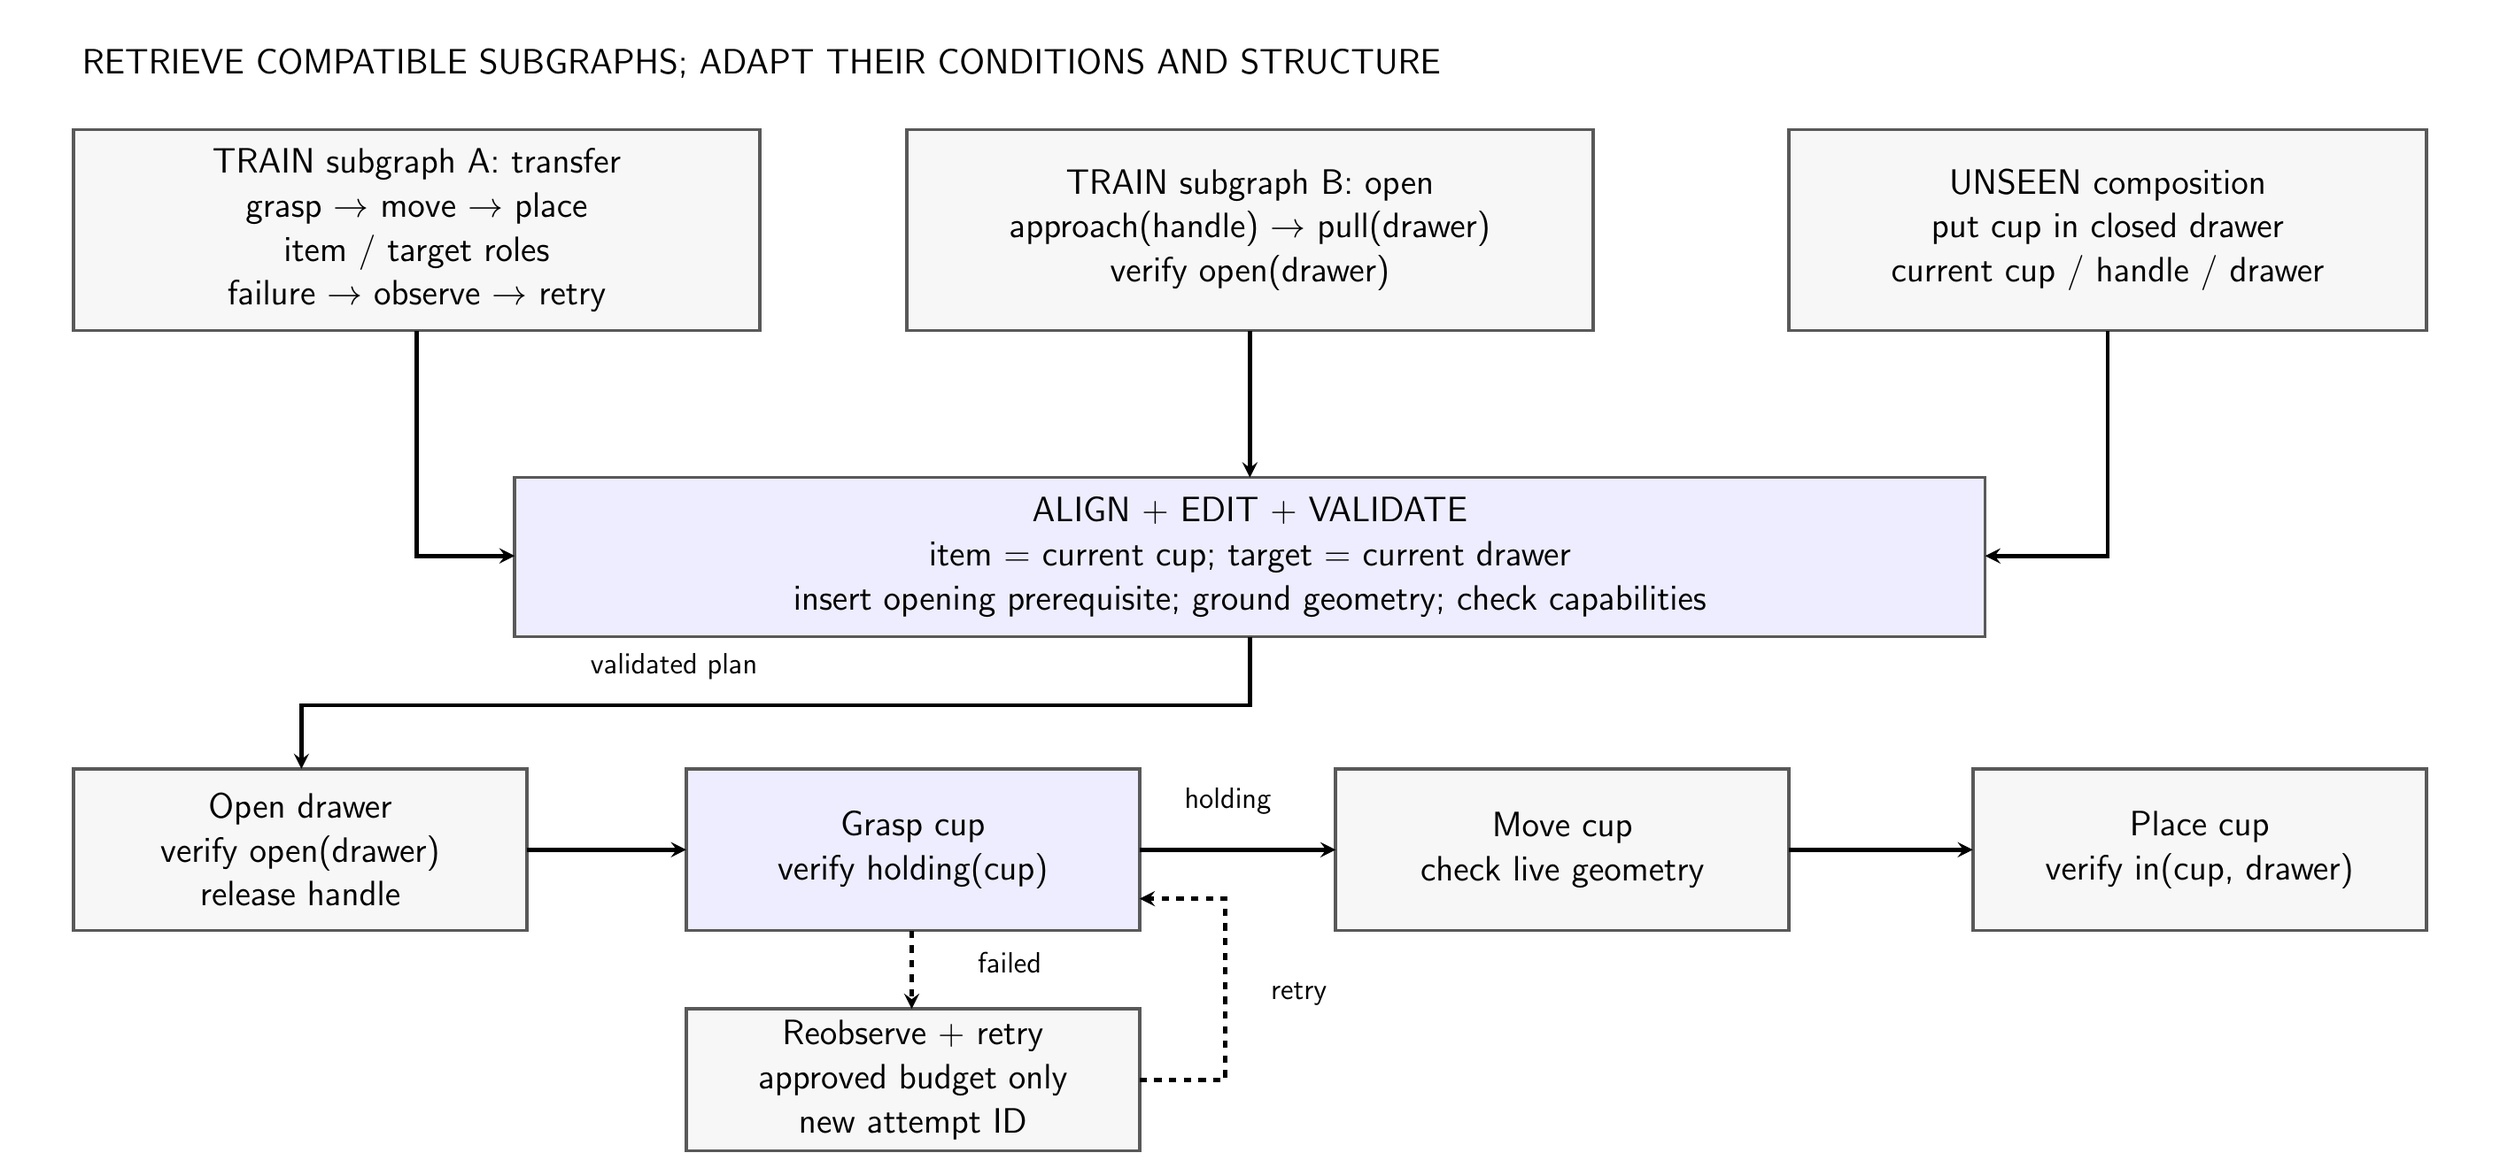
\begin{tikzpicture}[x=1pt,y=1pt,>=stealth]
\path[use as bounding box] (0,0) rectangle (1000,460);
\node[draw=black!65,fill=black!3,line width=1.3pt,minimum width=280pt,minimum height=82pt,text width=268pt,inner sep=4pt,align=center,font=\sffamily\fontsize{15}{18}\selectfont] (source1) at (160.0,376.0) {TRAIN subgraph A: transfer\\grasp $\rightarrow$ move $\rightarrow$ place\\item / target roles\\failure $\rightarrow$ observe $\rightarrow$ retry};
\node[draw=black!65,fill=black!3,line width=1.3pt,minimum width=280pt,minimum height=82pt,text width=268pt,inner sep=4pt,align=center,font=\sffamily\fontsize{15}{18}\selectfont] (source2) at (500.0,376.0) {TRAIN subgraph B: open\\approach(handle) $\rightarrow$ pull(drawer)\\verify open(drawer)};
\node[draw=black!65,fill=black!3,line width=1.3pt,minimum width=260pt,minimum height=82pt,text width=248pt,inner sep=4pt,align=center,font=\sffamily\fontsize{15}{18}\selectfont] (query) at (850.0,376.0) {UNSEEN composition\\put cup in closed drawer\\current cup / handle / drawer};
\node[draw=black!65,fill=blue!7,line width=1.3pt,minimum width=600pt,minimum height=65pt,text width=588pt,inner sep=4pt,align=center,font=\sffamily\fontsize{15}{18}\selectfont] (align) at (500.0,242.5) {ALIGN + EDIT + VALIDATE\\item = current cup; target = current drawer\\insert opening prerequisite; ground geometry; check capabilities};
\node[draw=black!65,fill=black!3,line width=1.3pt,minimum width=185pt,minimum height=66pt,text width=173pt,inner sep=4pt,align=center,font=\sffamily\fontsize{14}{18}\selectfont] (open) at (112.5,123.0) {Open drawer\\verify open(drawer)\\release handle};
\node[draw=black!65,fill=blue!7,line width=1.3pt,minimum width=185pt,minimum height=66pt,text width=173pt,inner sep=4pt,align=center,font=\sffamily\fontsize{14}{18}\selectfont] (grasp) at (362.5,123.0) {Grasp cup\\verify holding(cup)};
\node[draw=black!65,fill=black!3,line width=1.3pt,minimum width=185pt,minimum height=66pt,text width=173pt,inner sep=4pt,align=center,font=\sffamily\fontsize{14}{18}\selectfont] (move) at (627.5,123.0) {Move cup\\check live geometry};
\node[draw=black!65,fill=black!3,line width=1.3pt,minimum width=185pt,minimum height=66pt,text width=173pt,inner sep=4pt,align=center,font=\sffamily\fontsize{14}{18}\selectfont] (place) at (887.5,123.0) {Place cup\\verify in(cup, drawer)};
\node[draw=black!65,fill=black!3,line width=1.3pt,minimum width=185pt,minimum height=58pt,text width=173pt,inner sep=4pt,align=center,font=\sffamily\fontsize{14}{18}\selectfont] (retry) at (362.5,29.0) {Reobserve + retry\\approved budget only\\new attempt ID};
\draw[->,line width=1.7pt] (160,335) -- (160,243) -- (200,243);
\draw[->,line width=1.7pt] (500,335) -- (500,275);
\draw[->,line width=1.7pt] (850,335) -- (850,243) -- (800,243);
\draw[->,line width=1.7pt] (500,210) -- (500,182) -- (113,182) -- (113,156);
\node[fill=white,inner sep=2pt,font=\sffamily\fontsize{12}{14}\selectfont] at (265,198) {validated plan};
\draw[->,line width=1.7pt] (205,123) -- (270,123);
\draw[->,line width=1.7pt] (455,123) -- (535,123);
\node[fill=white,inner sep=2pt,font=\sffamily\fontsize{12}{14}\selectfont] at (491,143) {holding};
\draw[->,line width=1.7pt] (720,123) -- (795,123);
\draw[->,line width=1.7pt,dashed] (362,90) -- (362,58);
\node[fill=white,inner sep=2pt,font=\sffamily\fontsize{12}{14}\selectfont] at (402,77) {failed};
\draw[->,line width=1.7pt,dashed] (455,29) -- (490,29) -- (490,103) -- (455,103);
\node[fill=white,inner sep=2pt,font=\sffamily\fontsize{12}{14}\selectfont] at (520,64) {retry};
\node[anchor=base west,font=\sffamily\fontsize{14}{18}\selectfont] at (20,440) {RETRIEVE COMPATIBLE SUBGRAPHS; ADAPT THEIR CONDITIONS AND STRUCTURE};
\end{tikzpicture}}
\caption{Illustrative retrieval and adaptation for a new task: place a cup in a closed drawer. Two training subgraphs provide object transfer and drawer opening; the target composition is held out from the experience bank. Object roles are rebound to current observations, the open-drawer phase is inserted as a prerequisite, and current geometry supplies the action parameters. The adapted plan also incorporates an authorized recovery branch from historical failure evidence. The supervisor checks predicates and follows the approved branch; structural changes go to the planner. A failed grasp appends a failed event to $X$ and creates a distinct retry instance, rather than relabeling the failed action as successful. The example explains graph composition and revision; it makes no claim that this task has been implemented or solved.}
\label{fig:adaptation}
\end{figure*}
